% This is a template for the title page of any assignment or report.
% Owner: Bratin Mondal
% Usage:
% 1. Replace the placeholders with your information.
% 2. Add any additional information, if needed.
% 3. Add your university logo or any other image.
% 4. Add any other details, if needed, below the image.
% 5. Compile the document to see the output.

\documentclass[12pt]{article}
\usepackage{graphicx}
\usepackage{comment}
\usepackage{booktabs}
\usepackage{amsmath} % For mathematical formulas
\usepackage{algorithm} % For pseudocode
\usepackage{algpseudocode} % For pseudocode
\usepackage{lipsum} % For dummy text

\usepackage{geometry}
\usepackage{hyperref}
\usepackage{pgfplots}
\usepackage{float}
\renewcommand{\rmdefault}{ptm}
\newcommand{\bmr}[1]{\textcolor{red}{#1}}
\newcommand{\bmg}[1]{\textcolor{green}{#1}}
\newcommand{\bmb}[1]{\textcolor{blue}{#1}}
\newcommand{\bmp}[1]{\textcolor{magenta}{#1}}

% Define macros for information
\newcommand{\myName}{Bratin Mondal}
\newcommand{\myRollNumber}{21CS10016}
\newcommand{\myCourse}{CS60050 - Machine Learning}
\newcommand{\myAssignment}{3}
\newcommand{\myAssignmentTitle}{Country Grouping using Complete Linkage Divisive (Top-Down) Clustering Technique}
\newcommand{\myUniversity}{Indian Institute of Technology Kharagpur}
\geometry{a4paper, margin=0.5in} % Adjust margins if necessary
\begin{document}
	
	\begin{titlepage}
		\centering
		
		{\Huge{\textbf{\myCourse}}}
		\vspace{0.5cm}
		
		{\Huge{Assignment \myAssignment}}
		
		\vspace{2cm}
		
		% Add your university logo or any other image here
		\includegraphics[width=0.5\textwidth]{iit_kgp_logo.png}
		
		\vspace{2cm}
		
		% Add your report title here
		{\Huge\textbf{\myAssignmentTitle}}
		
		\vspace{2cm}
		
		% Add any other details like your name, date, etc.
		{\Large\textbf{\myName}} 
		\vspace{0.2cm}
		
		\large{\myRollNumber}    
		\vspace{2cm}
		
		% Add any additional information, if needed
		{\large\textit{Department of Computer Science and Engineering,}}
		
		{\large\textit{\myUniversity}}
		\vspace{0.3cm}
		
		% Two lines above the image
		\hrule 
		\vspace{0.5cm}
		
		% Add any other details, if needed, below the image
		
	\end{titlepage}
	
	\section{Problem Statement}
	\begin{itemize}
		\item Implement K-means clustering algorithm from scratch for $k=3, 4, 5, 6$.
		\item Find the optimal value of $k$ using the silhouette coefficient metric.
		\item Implement Complete Linkage Divisive (Top-Down) Clustering Technique from scratch for the optimal value of $k$ found in previous step.
		\item Establish a one-to-one correspondence between the clusters obtained from K-means and Complete Linkage Divisive (Top-Down) Clustering Technique and calculate the Jaccard Similarity.
	\end{itemize}

	\section{Model Description}

	\subsection{K-means Clustering Algorithm:}
	\textbf{Algorithm:} \\
	\begin{algorithmic}
	\State Initialize $K$ cluster centroids randomly
	\Repeat
		\State Assign each data point to the nearest centroid
		\State Update each centroid as the mean of the data points assigned to it
	\Until{Convergence}
	\end{algorithmic}
	
	\subsection{Silhouette Coefficient:}
	\textbf{Formula:}
	\[
	s(i) = \frac{b(i) - a(i)}{\max\{a(i), b(i)\}}
	\]
	where,
	\begin{itemize}
		\item $s(i)$ is the silhouette coefficient of object $i$
		\item $a(i)$ is the average distance from $i$ to other objects in the same cluster
		\item $b(i)$ is the average distance from $i$ to objects in the nearest cluster that $i$ is not a part of
	\end{itemize}
	
	\subsection{Complete Linkage Divisive (Top-Down) Clustering Technique:}
	\textbf{Pseudocode:} \\
	\begin{algorithmic}
	\State Start with all data points in one cluster
	\State Until the desired number of clusters is reached:
	\State \quad Find the cluster with the maximum diameter to split
	\State \quad Split the cluster into two based on the farthest points
	\State \quad Update the cluster assignments
	\end{algorithmic}
	
	\subsection{Jaccard Similarity:}
	\textbf{Formula:}
	\[
	J(A, B) = \frac{|A \cap B|}{|A \cup B|}
	\]
	where,
	\begin{itemize}
		\item $J(A, B)$ is the Jaccard similarity coefficient between sets $A$ and $B$
		\item $|A \cap B|$ is the size of the intersection of sets $A$ and $B$
		\item $|A \cup B|$ is the size of the union of sets $A$ and $B$
	\end{itemize}

	\subsection{Cosine Similarity:}
	\textbf{Formula:}
	\[
	\text{cosine\_similarity}(A, B) = \frac{A \cdot B}{\|A\| \|B\|}
	\]
	where,
	\begin{itemize}
		\item $\text{cosine\_similarity}(A, B)$ is the cosine similarity between vectors $A$ and $B$
		\item $A \cdot B$ is the dot product of vectors $A$ and $B$
		\item $\|A\|$ and $\|B\|$ are the Euclidean norms of vectors $A$ and $B$ respectively
	\end{itemize}
	
	
	\section{Results}
	\subsection{K-means Clustering}
	The optimal value of $k$ was found to be 3 using the silhouette coefficient metric. 
	\begin{table}[htbp]
		\centering
		\begin{tabular}{cc}
			\toprule
			\textbf{Value of K} & \textbf{Silhouette Coefficient} \\
			\midrule
			3 & 0.6988985969993166 \\
			4 & 0.6137622384616047 \\
			5 & 0.5641146777848881 \\
			6 & 0.4879572689267768 \\
			\bottomrule
		\end{tabular}
		\caption{Silhouette Coefficients for Different Values of K}
		\label{tab:silhouette}
	\end{table}
	We observe that the silhouette coefficient decreases as the value of $k$ increases. Hence, the optimal value of $k$ is 3. Analysing the change of silhouette coefficient with respect to $k$ is shown below
	\begin{figure}[H]
		\centering
		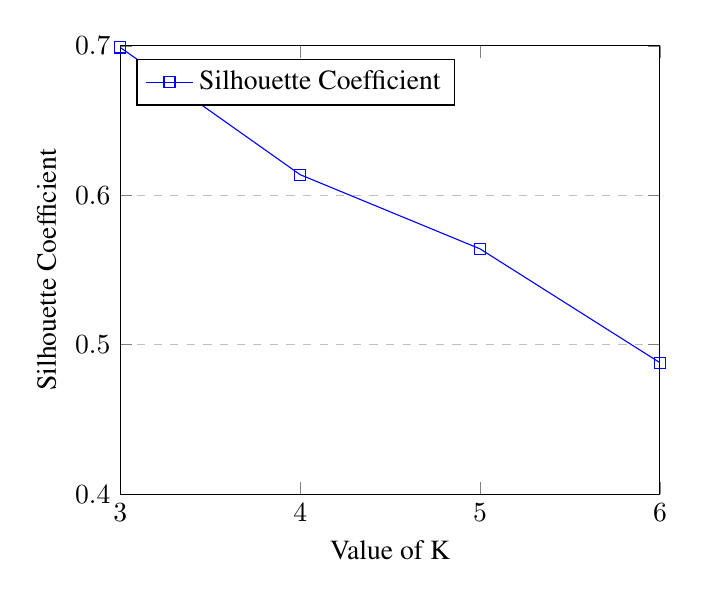
\begin{tikzpicture}
			\begin{axis}[
				xlabel={Value of K},
				ylabel={Silhouette Coefficient},
				xmin=3, xmax=6,
				ymin=0.4, ymax=0.7,
				xtick={3,4,5,6},
				ytick={0.4,0.5,0.6,0.7},
				legend pos=north west,
				ymajorgrids=true,
				grid style=dashed,
			]
			
			\addplot[
				color=blue,
				mark=square,
				]
				coordinates {
					(3, 0.6988985969993166)
					(4, 0.6137622384616047)
					(5, 0.5641146777848881)
					(6, 0.4879572689267768)
				};
				\legend{Silhouette Coefficient}
			\end{axis}
		\end{tikzpicture}
		\caption{Silhouette Coefficients for Different Values of K}
		\label{fig:silhouette_plot}
	\end{figure}
	The decrease in silhouette coefficient with increasing \( k \) suggests that the clusters become less distinct as more clusters are introduced. This indicates that the data may not naturally divide into more than three clusters, leading to a decrease in the quality of clustering as \( k \) increases.
	\subsection{Complete Linkage Divisive (Top-Down) Clustering Technique}
	The Silhouette Coefficient for the optimal value of \( k \) was found to be 0.6895572393550293.
	
	This high Silhouette Coefficient indicates that the clusters formed by the Complete Linkage Divisive clustering technique are well-separated and dense, with each data point closely resembling its own cluster centroid compared to others. It suggests that the chosen value of \( k \) effectively captures the underlying structure of the data. However, further analysis and validation may be necessary to ensure the robustness and generalizability of the clustering results.
	
	\subsection{Jaccard Similarity}
	The Jaccard Similarity between the clusters obtained from K-means and Complete Linkage Divisive (Top-Down) Clustering Technique is shown in the Table below.
	
	\begin{figure}[h]
		\centering
		\includegraphics[width=0.8\textwidth]{jaccard_similarity.png} % Provide the file name or path to the image
		\caption{Jaccard Similarity}
		\label{fig:example}
		\end{figure}

	\begin{table}[htbp]
		\centering
		\begin{tabular}{ccc}
			\toprule
			\textbf{K-Means Cluster Index} & \textbf{Divisive Cluster Index} & \textbf{Jaccard Similarity} \\
			\midrule
			1 & 1 & 0.8787878787878788 \\
			2 & 3 & 0.8315789473684211 \\
			3 & 2 & 0.6610169491525424 \\
			\bottomrule
		\end{tabular}
		\caption{Comparison of K-Means and Divisive Clustering Indices with Jaccard Similarity}
		\label{tab:cluster_comparison}
	\end{table}
	
	The Jaccard Similarity measures the similarity between two sets by comparing their intersection to their union. In the context of clustering, it quantifies the similarity of cluster assignments between different clustering techniques. 
	
	From Table \ref{tab:cluster_comparison}, we observe that the Jaccard Similarity values range between 0.66 and 0.88, indicating moderate to high similarity between the cluster assignments produced by K-means and Complete Linkage Divisive clustering. Higher Jaccard Similarity values suggest a greater agreement between the clustering results of the two techniques.
	
	However, it's essential to note that while Jaccard Similarity provides valuable insights into the agreement between clustering results, it does not account for the structure or quality of the clusters themselves. Therefore, further analysis, such as examining the cluster centroids or silhouette scores, may be necessary to fully assess the clustering performance.


\section{Analysis}

Table \ref{tab:time_taken} shows the time taken for each step of the process. The "Load Data" step, which involves loading the dataset, took a minimal amount of time, while steps such as "Find Best K" and "Hierarchical Clustering" required more computation. 

The total time taken for all steps was \textbf{2.0712053775787354} seconds.

This breakdown of time taken for each step provides valuable insights into the computational overhead of the process and can help identify potential bottlenecks or areas for optimization.

\begin{table}[htbp]
    \centering
    \begin{tabular}{cc}
        \toprule
        \textbf{Step} & \textbf{Time Taken (seconds)} \\
        \midrule
        Load Data & 0.0031189918518066406 \\
        Clustering with K = 3 & 0.26228976249694824 \\
        Clustering with K = 4 & 0.24265837669372559 \\
        Clustering with K = 5 & 0.25972580909729004 \\
        Clustering with K = 6 & 0.27604103088378906 \\
        Find Best K & 1.0408053398132324 \\
        Hierarchical Clustering & 1.0254216194152832 \\
        Calculate Jaccard Similarity & 0.0003230571746826172 \\
        \midrule
        \textbf{Total Time Taken} & \textbf{2.0712053775787354} \\
        \bottomrule
    \end{tabular}
    \caption{Time Taken for Each Step}
    \label{tab:time_taken}
\end{table}

\section{Conclusion}

In this study, we implemented the K-means clustering algorithm from scratch for \( k = 3, 4, 5, 6 \) and found the optimal value of \( k \) to be 3 using the silhouette coefficient metric. We also implemented the Complete Linkage Divisive (Top-Down) Clustering Technique for the optimal value of \( k \) and obtained a high Silhouette Coefficient, indicating well-separated and dense clusters.

Additionally, we established a one-to-one correspondence between the clusters obtained from K-means and Complete Linkage Divisive clustering and calculated the Jaccard Similarity. The moderate to high Jaccard Similarity values suggested a reasonable agreement between the cluster assignments produced by the two techniques.

Furthermore, the breakdown of time taken for each step provided valuable insights into the computational overhead of the process. Steps such as finding the best \( k \) and performing hierarchical clustering contributed significantly to the total computation time.

Overall, this analysis sheds light on the effectiveness and efficiency of different clustering techniques in partitioning data and provides a foundation for further exploration and optimization in future studies.



\end{document}